\subsection{Image Processing}
In the previous sections we have learned about two different approaches to train neural nets on solving certain tasks. Although we came to understand that the complexity of the task to be solved correlates strongly with the amount of data at hand, there exist domains from which it is undeniably easier to do so. To equip a neural net with some sort of prior knowledge by switching the domain may therefore not only be highly desirable but sometimes also needed if the amount or quality of data is not sufficient. One domain which is of special interest when it comes to interacting in a three dimensional environment is a domain that represents depth information. If there are any, it may sometimes be possible to extract this kind of prior knowledge from a depth camera. As for this work, we need to rely on stereo cameras and powerful algorithms that allow us to compute depth images in real time. The algorithm that helps us to do so, in terms of the extraction of weighted least squares disparity maps \cite{min2014fast}, will be presented in the following paragraph - Depth Map Extraction.
\subsubsection{Depth Map Extraction}
As already pointed out, the depth map is generated from stereo camera images by a technique called stereo block matching \cite{hamzah2010sum}. This method works best for edge filtered images, as will become clear soon. To obtain edge filtered images $\bm{E}$, the stereo RGB images are first converted into grayscale $\bm{G}$, which are then convolved with the Sobel kernel $\bm{S}_x$ along the horizontal axis \cite{sobel2014an} (equation \ref{eq::323_sobel_conv}, figure \ref{fig::323_image_preprocessing}). 
\begin{align}
	\bm{E} = \bm{S}_x*\bm{G}
	\label{eq::323_sobel_conv}
\end{align}
\begin{figure}[h]
	\centering
	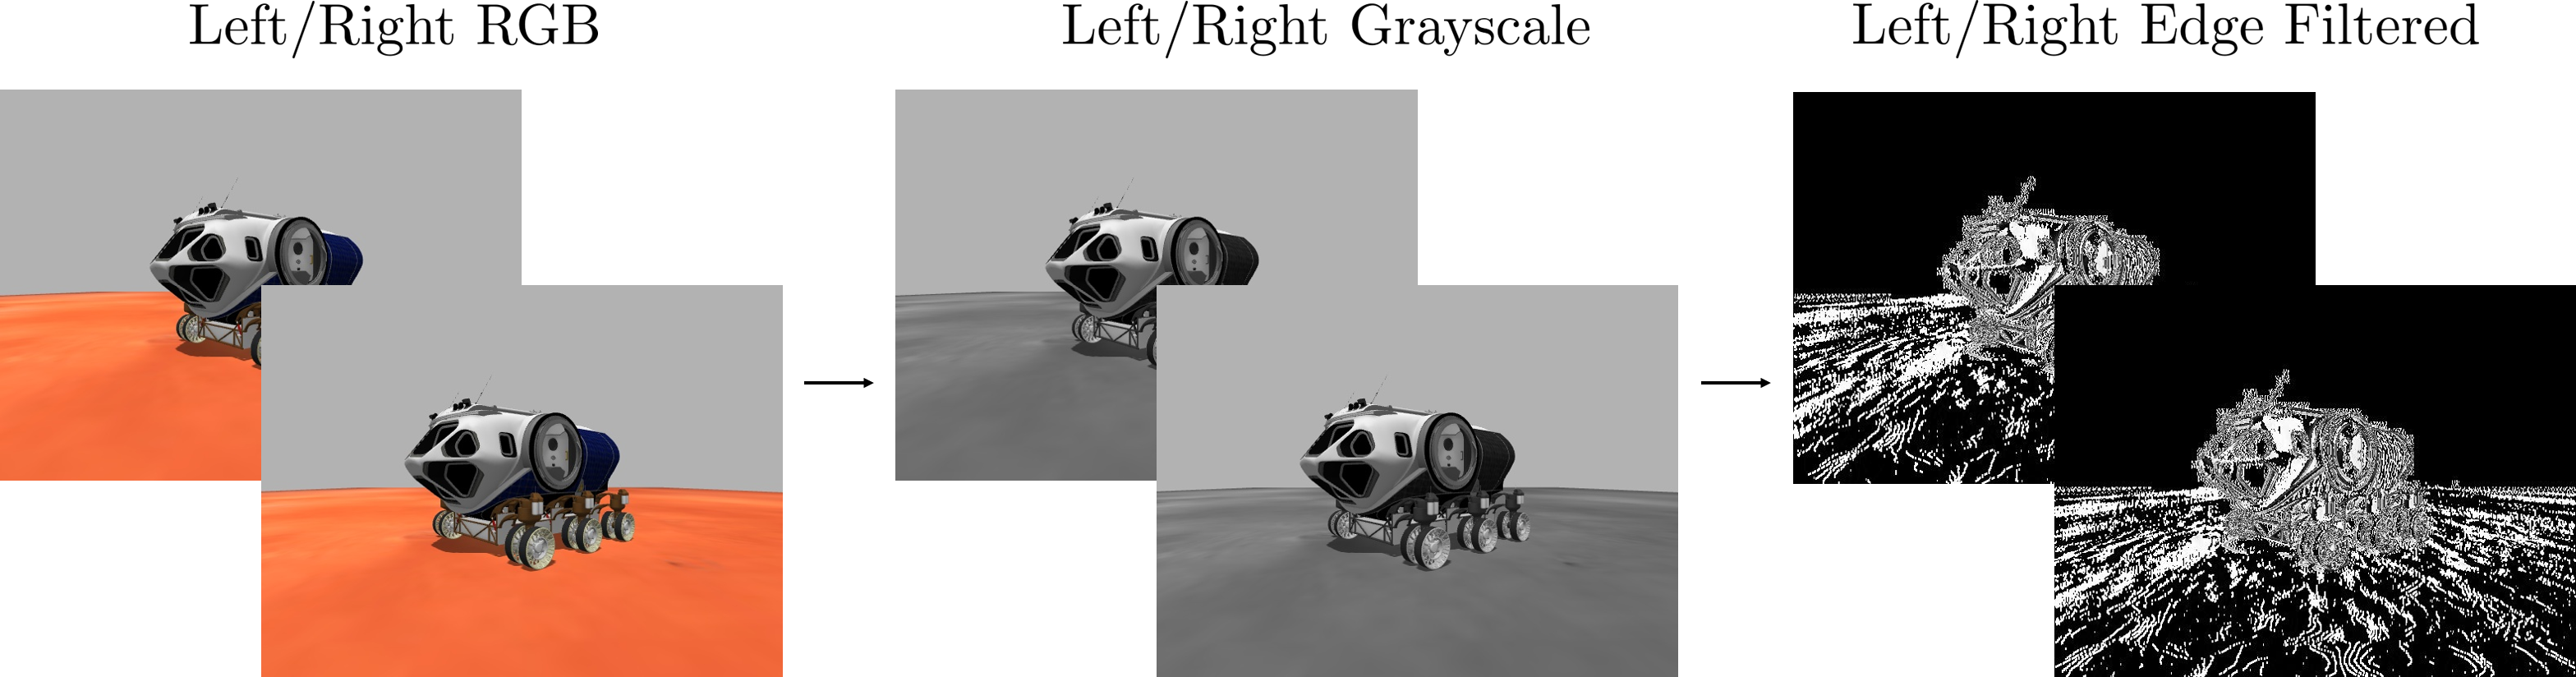
\includegraphics[scale=.28]{chapters/03_background/img/image_preprocessing.png}
	\caption{Image preprocessing to obtain edge filtered images. The images were taken within the simulation environment Gazebo (\href{http://gazebosim.org/}{link}), and show a space exploration vehicle, for which, with the friendly support of NASA, we generated a Gazebo version (\href{https://github.com/mhubii/gazebo_models}{link}).}
	\label{fig::323_image_preprocessing}
\end{figure}
When having a look at the Sobel kernel $\bm{S}_x$ (equation \ref{eq::323_sobel}), it immediately becomes clear that it approximates the derivative of an image along the horizontal axis. Therefore, at locations of steep change, or simply put, edges, the convolution of the grayscale images with the Sobel kernel results in high values, and thus in the typical appearance of an edge filtered image.
\begin{align}
	\bm{S}_x=
	\begin{pmatrix}
		-1 & 0 & +1 \\
		-2 & 0 & +2 \\
		-1 & 0 & +1
	\end{pmatrix}
	\label{eq::323_sobel}
\end{align}
To understand the block matching algorithm, we first need to figure out the transformation that images undergo for a change in perspective, which is caused by the two different positions of the cameras within the stereo camera pair. For an ideal setup, we have two identical cameras, and they are neither rotated relatively to each other, nor is there any other translation, but a shift along the x-axis (figure. \ref{fig::323_stereo_camera}). This may of course not always be true, and there are methods to correct for uncertainties, which we will present in the following paragraph, but omit for simplicity right now. The principle goal, for the inference of depth information from two images, is to find points in the right image that correspond to points in the left image. By triangulation, the displacement or disparity of a point in the right image, relative to its corresponding point in the left image, can then be used to extract the depth. The farther a point $\bm{X}$ lies away from the cameras, the smaller its displacement will be. In figure \ref{fig::323_stereo_camera}, we can see that a point $\bm{X}$, which is seen by the left camera, could in principle lie anywhere on the epipolar line at $\bm{x}'$, as seen from the right camera, if there is no depth information available. 
\begin{figure}[h]
	\centering
	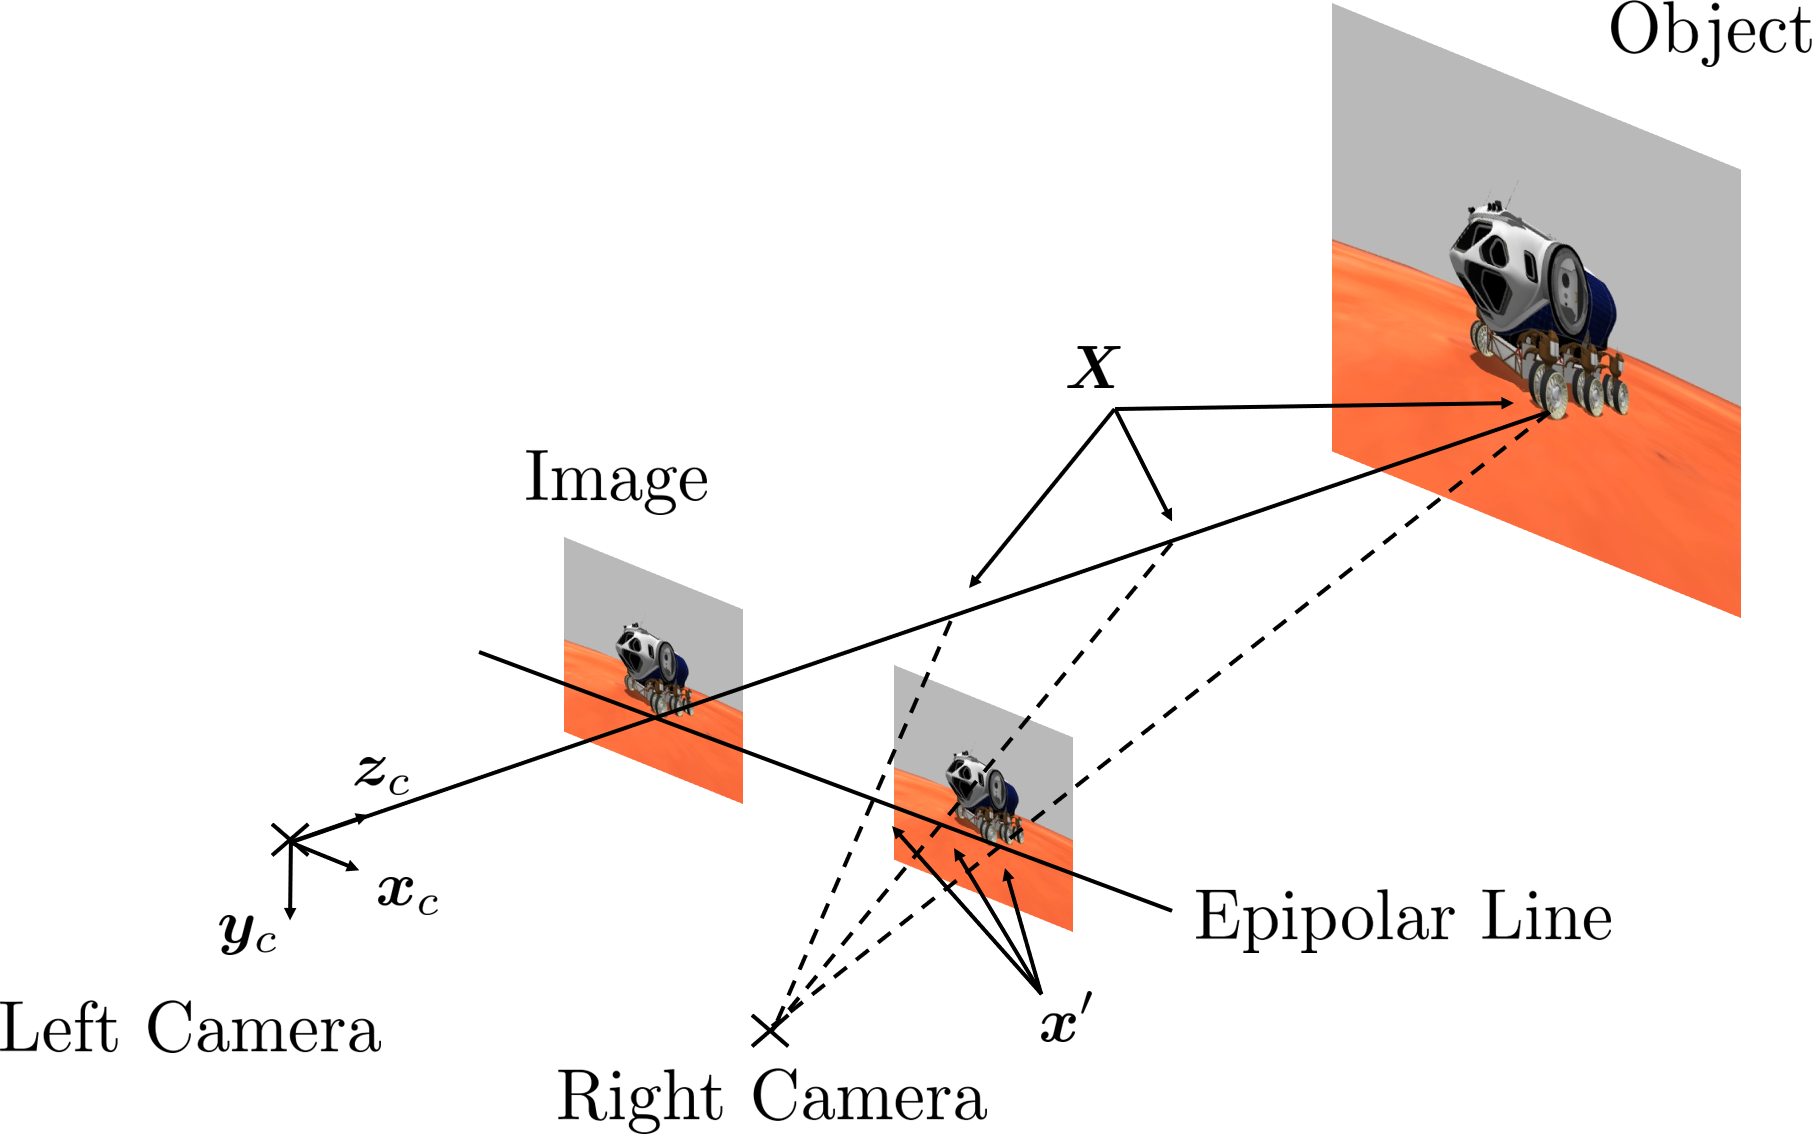
\includegraphics[scale=.28]{chapters/03_background/img/stereo_camera.png}
	\caption{The stereo setup with a left and a right camera.}
	\label{fig::323_stereo_camera}
\end{figure}
It results that, to find correspondences, one only has to search along the epipolar line. Also, since points in the right image that correspond to points in the left image, will always be displaced to the left, one only has to search in this direction. The procedure is shown in figure \ref{fig::323_left_disparity_map}. Instead of looking for single pixel correspondences, it is advised to search for whole block correspondences, since it reduces the noise drastically. Blocks of a defined block size $N$ are taken from the left image, and then the sum of absolute differences SAD is computed for every displacement $d$ in the right image, ranging from zero to number of disparities $D$ (equation \ref{eq::323_sad}, figure \ref{fig::323_left_disparity_map}).
\begin{align}
	\text{SAD}(d) = \sum_{x,y=0}^N |\bm{E}_\text{left}(x,y) - \bm{E}_\text{right}(x-d,y)|
	\label{eq::323_sad}
\end{align}
The disparity $d$ that minimizes the sum of absolute differences SAD is taken to serve as the best correspondence and is therefore used in the disparity map.  Here we can already see that due to the uniqueness of the edge filtered the images $\bm{E}$, it is easier to find correspondences there, rather than in the grayscale or RGB images.
\begin{figure}[h]
	\centering
	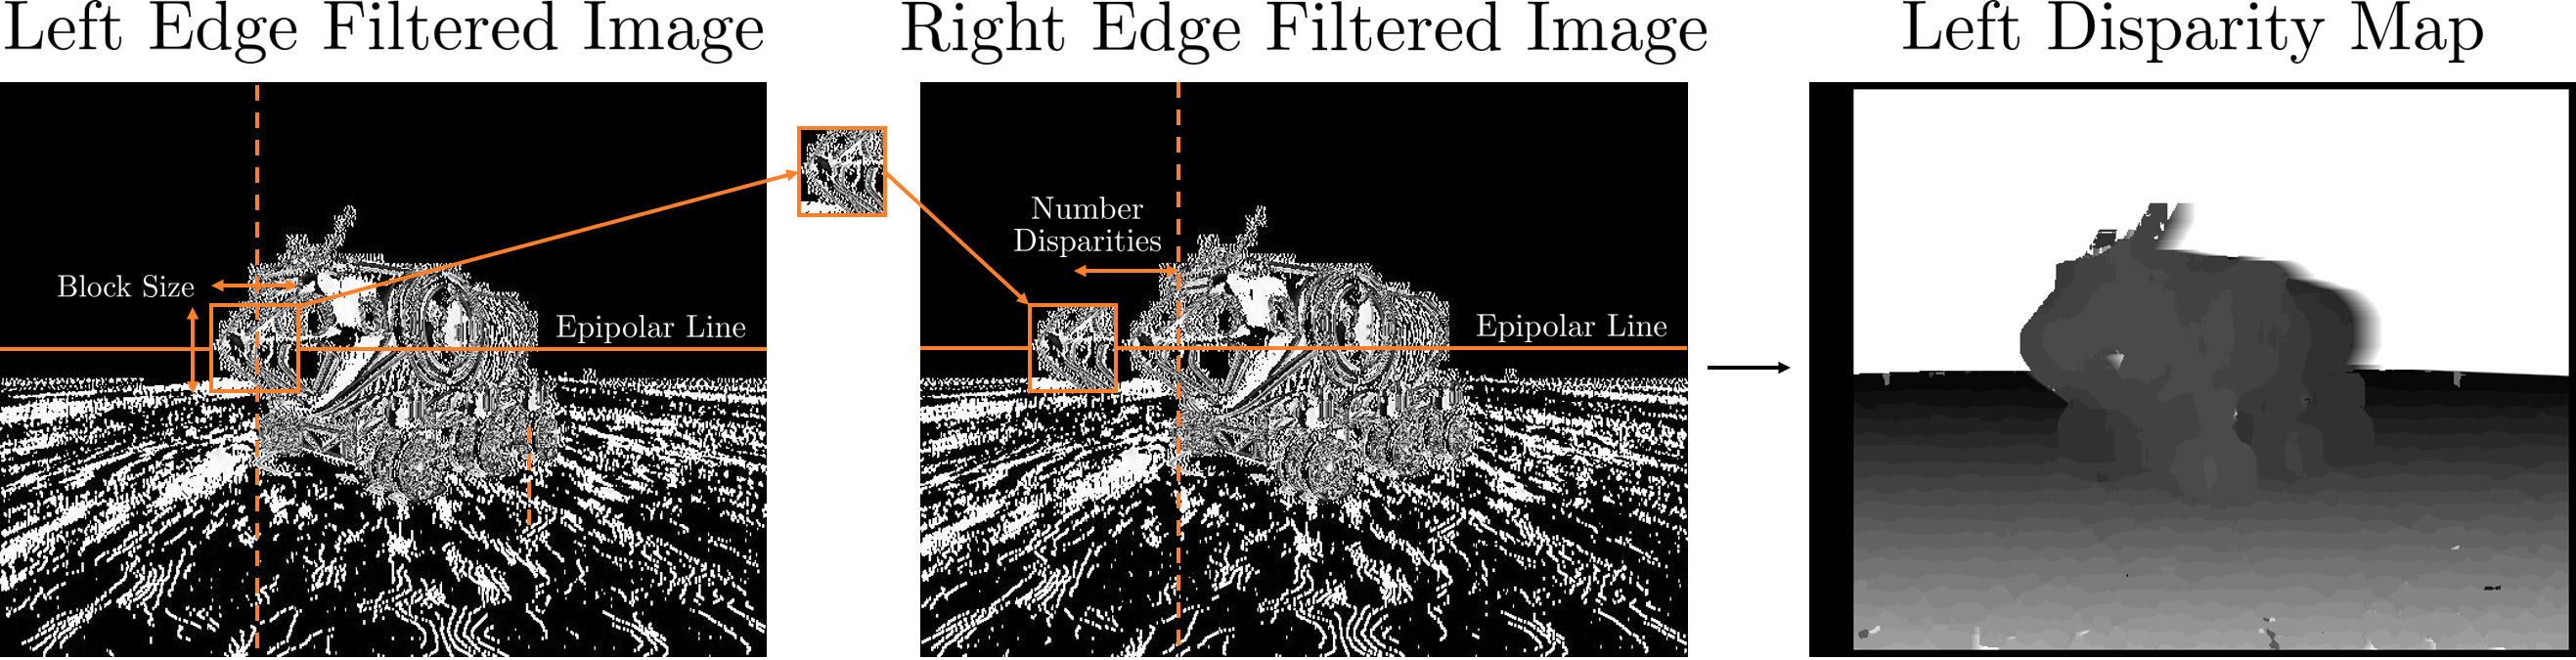
\includegraphics[scale=.28]{chapters/03_background/img/left_disparity_map.png}
	\caption{Generation of the left disparity map by the block matching algorithm.}
	\label{fig::323_left_disparity_map}
\end{figure}
To further refine the disparity map, and especially to assure good results in textureless  regions, we apply a weighted least squares filtering, which is based on the confidence of depth measures. The confidence of depth measures is obtained from the variance within the disparity map $\bm{D}$ (equation \ref{eq::323_variance}, figure \ref{fig::323_confidence_map}).
\begin{align}
	 \text{Var}(\bm{D}) = \text{E}\left[\bm{D}^2\right] - \text{E}\left[\bm{D}\right]^2
	\label{eq::323_variance}
\end{align} 
Therein, the expectation value for $\bm{D}$ is computed by a convolution with the kernel $\bm{K}$ from the following equation
\begin{align}
	\bm{K} &= \alpha
	\begin{pmatrix}
	1 & \dots & 1 \\
	\vdots & \ddots & \vdots \\
	1 & \dots & 1
	\end{pmatrix} \\
	\text{E}\left[\bm{D}\right] &= \bm{K}*\bm{D},
	\label{eq::323_kernel}
\end{align}
where $\alpha = \frac{1}{\text{width}\cdot\text{height}}$ is the normalization factor. The expectation value of the disparity map squared $\text{E}\left[\bm{D}^2\right]$ is computed in the same way, except for that all elements are squared prior to summing them up. Given the variance, we can introduce a concept which is named confidence map. The confidence map $\text{Con}(\bm{D})$ is a measure for the certainty of the computed disparity, and is defined to be linearly dependent on the variance as follows
\begin{align}
	\text{Con}(\bm{D}) = \max\left(1-r\text{Var}(\bm{D}),0\right),
\end{align}
where $r$ is a roll-off factor that defines the change of confidence with growing variance. The resulting disparity confidence is shown in figure \ref{fig::323_confidence_map}, and is used to outweigh outlying disparity values from the final weighted least squares disparity map. 
\begin{figure}[h]
	\centering
	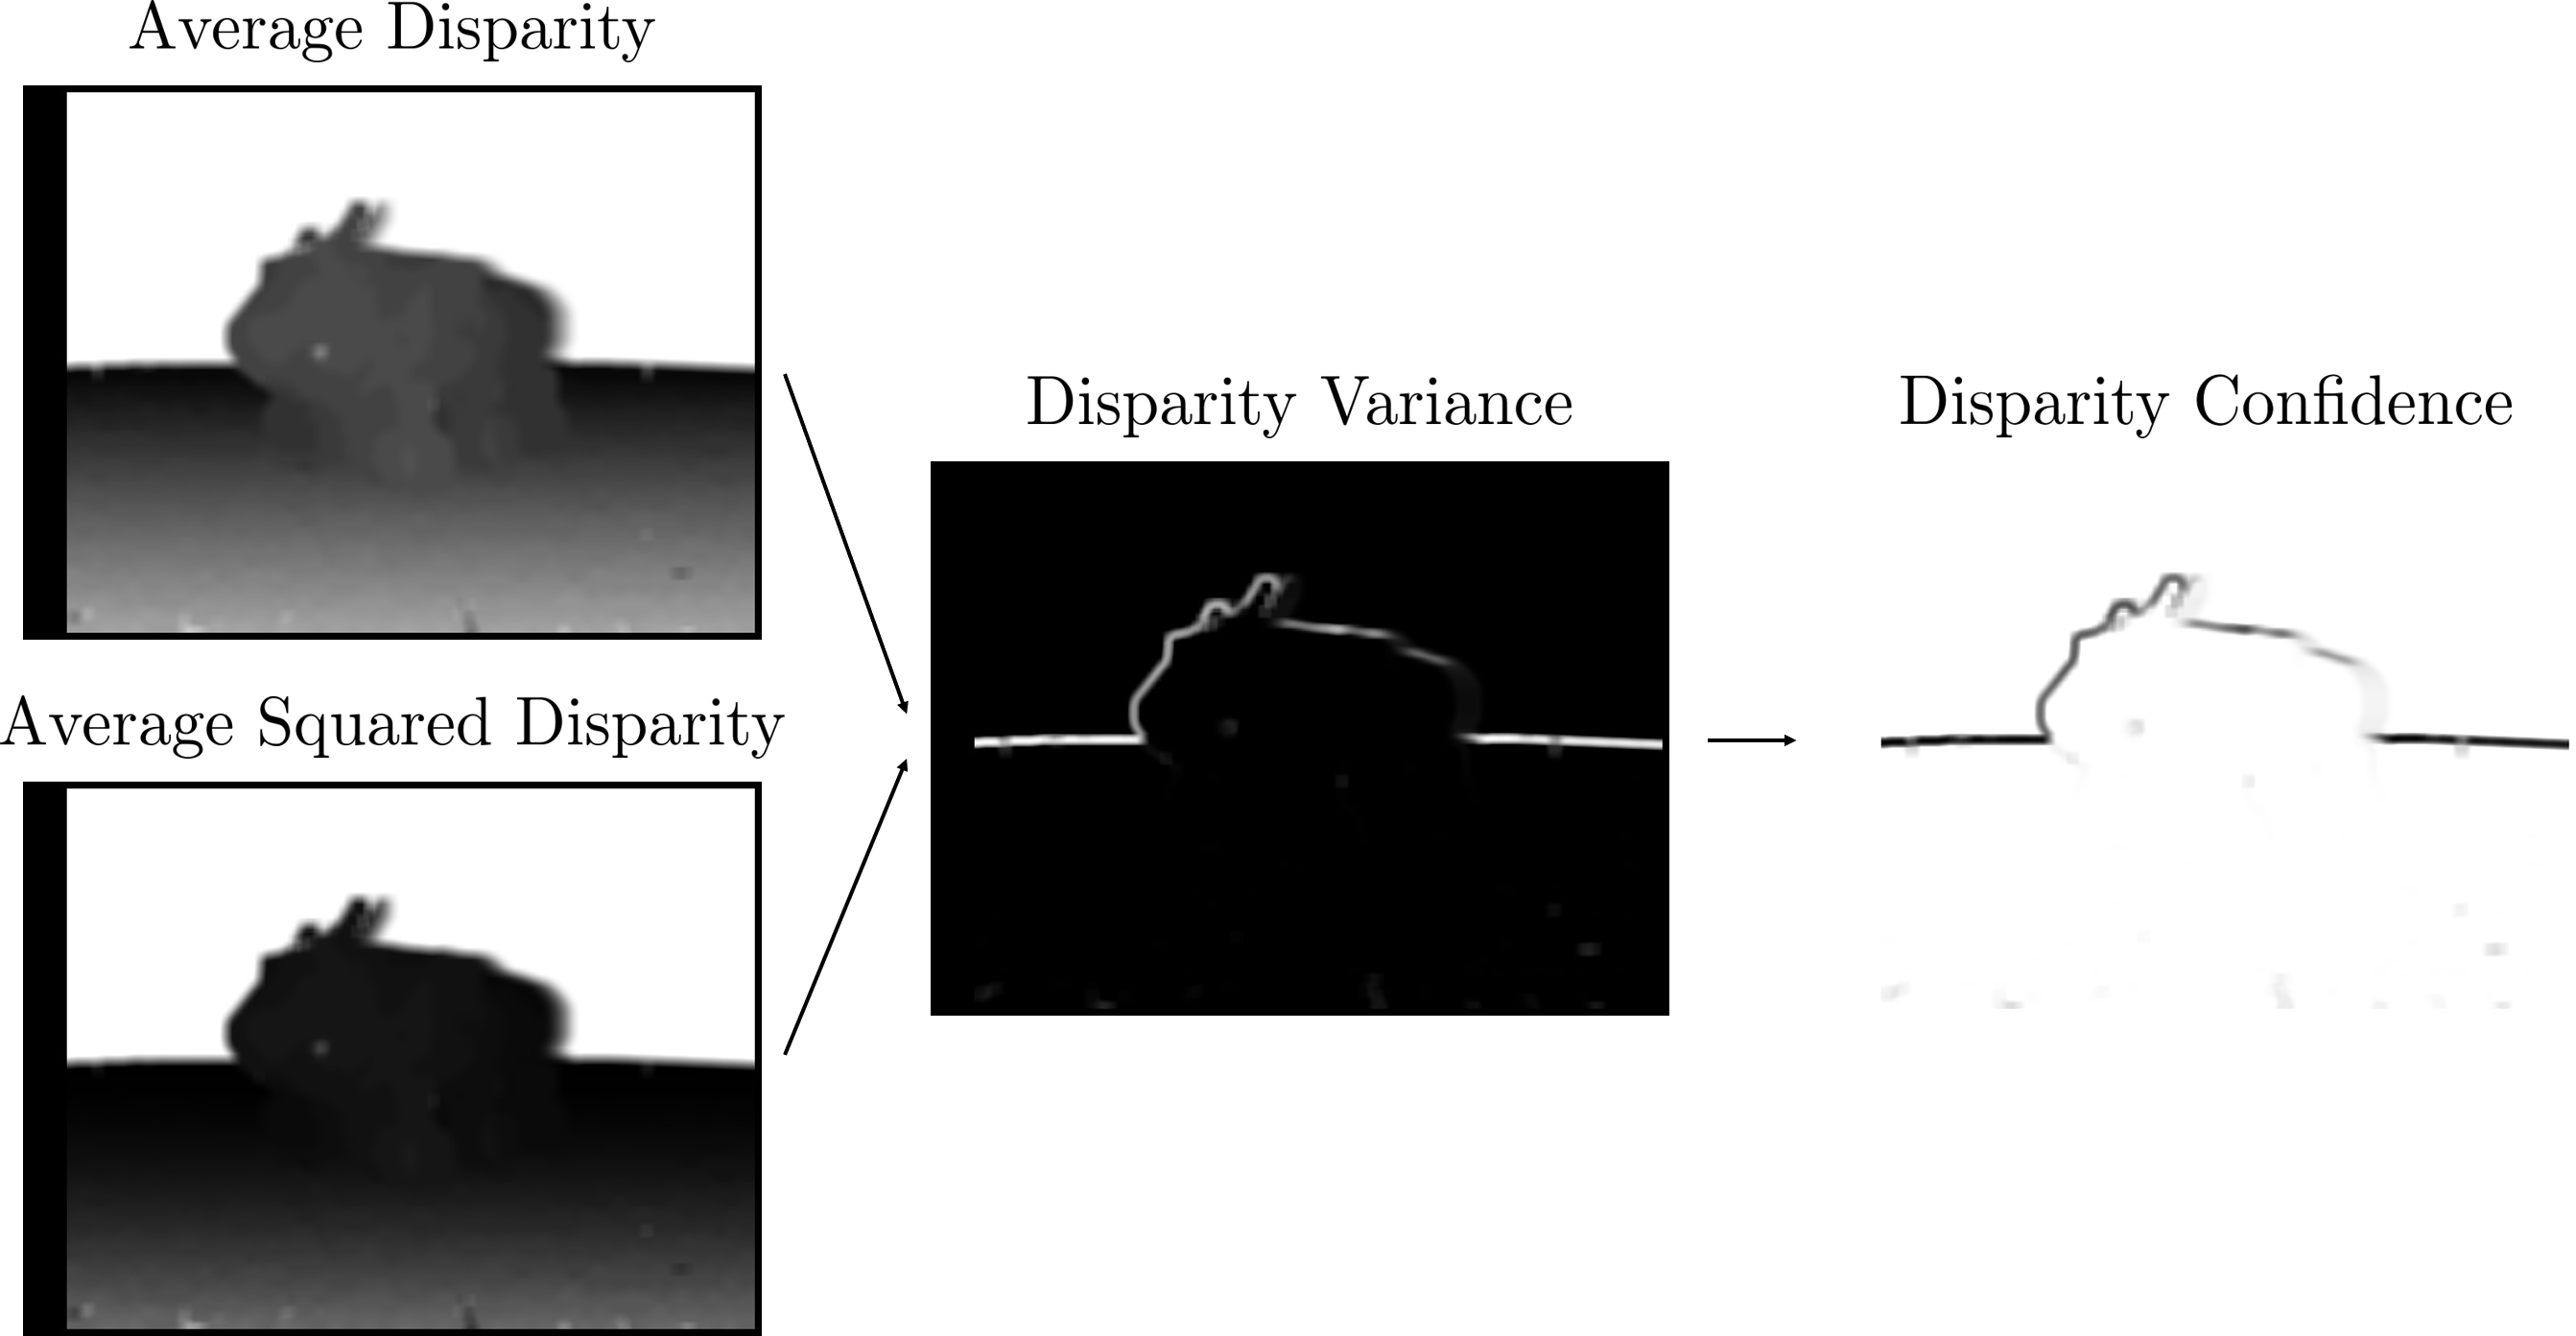
\includegraphics[scale=.28]{chapters/03_background/img/confidence_map.png}
	\caption{Generation of the confidence map from the variance within the disparity map.}
	\label{fig::323_confidence_map}
\end{figure}
Prior to that, we further introduce an additional measure for the prevention of accidentally assigned correspondences in the initial block matching algorithm by using a left right consistency check \cite{egnal2004stereo}. Therefore, the block matching algorithm is used on the right image, and we search for correspondences in the left image. In contrast to the computation of the left disparity map $\bm{D}_\text{left}$, for the right disparity map $\bm{D}_\text{right}$, we only need to check for correspondences along the epipolar line in the positive displacement direction. The left right consistency $\bm{L}$ is then obtained by 
\begin{align}
	\bm{L}(x, y) = 
	\begin{cases}
	\min \left[\text{Con}(\bm{D}_\text{left})(x, y), \text{Con}(\bm{D}_\text{right})(x + d_\text{left}, y)\right] & \text{for } \Delta d < t  \\
	0 & \text{else}
	\end{cases},
\end{align}
where $d_\text{left}$ is the disparity of $\bm{D}_\text{left}$ at position $(x,y)$, and therefore represents the index shift which results from the block matching algorithm. Furthermore, if $\Delta d = \bm{D}_\text{left}(x, y) + \bm{D}_\text{right}(x + d_\text{left}, y)$ is smaller than a threshold $t$, then the left right consistency $\bm{L}$ is taken to be the lower bound approximation of the left and right confidences. Otherwise, the consistency is taken to be false, and hence zero (figure \ref{fig::323_weighted_least_squares_disparity}). As already pointed out, the left right consistency, which is nothing but a confidence measure, usually reveals uncertainties in textureless regions. The weighted least squares filtering that we are about to present uses this fact to its advantage. In a first step, a consistency weighted disparity map $\bm{C}$ is computed via equation \ref{eq::323_cwd} (figure \ref{fig::323_weighted_least_squares_disparity}).
\begin{align}
	\bm{C}=\bm{L}\cdot\bm{D}_\text{left},
	\label{eq::323_cwd}
\end{align}
where $\cdot$ is an element-wise multiplication. Further, the weighted least squares filter is based on the idea of a bilateral filter \cite{tomasi1998bilateral}, and it will try to minimize an energy function $J(\bm{U})$, which takes the original grayscale image as guidance to compute a weight $w_{p,q}$ for neighboring pixels $p$, and $q$ as follows
\begin{align}
	w_{x,y,i,j}(g) = exp(-|g_{x,y}-g_{i,j}|/\sigma).
	\label{eq::323_weight}
\end{align}
Depending on the range parameter $\sigma$, this weight will be high for similar neighboring pixels of the grayscale image $g$, and therefore lead to huge costs in the following energy function $J(\bm{U})$ that we try to minimize
\begin{align}
	J(\bm{U}) = \sum_{x,y}\left[(u_{x,y}-c_{x,y})^2+\lambda\sum_{(i,j)\in\mathcal{N}(x,y)}w_{x,y,i,j}(g)(u_{x,y}-u_{i,j})^2\right],
\end{align}
where $c_{x,y}$ are single pixels of the consistency weighted disparity map. The formulation of this energy function results in a solution $\bm{U}$ that encourages the propagation of disparity values from high- to low-confidence regions (figure \ref{fig::323_weighted_least_squares_disparity}). Additionally, the weight $w$, together with the smoothing parameter $\lambda$, ensure to have similar disparity values in regions with similar texture. The final disparity map $\bm{D}_\text{final}$ is then obtained by normalizing the resulting image $\bm{U}$ with
\begin{align}
	\bm{D}_\text{final} = \frac{\bm{U}}{\text{WLS}(\bm{L})},
\end{align}
where $\text{WLS}(\bm{U})$ is the weighted least squares filtered version of the left right consistency $\bm{L}$.
\begin{figure}[h]
	\centering
	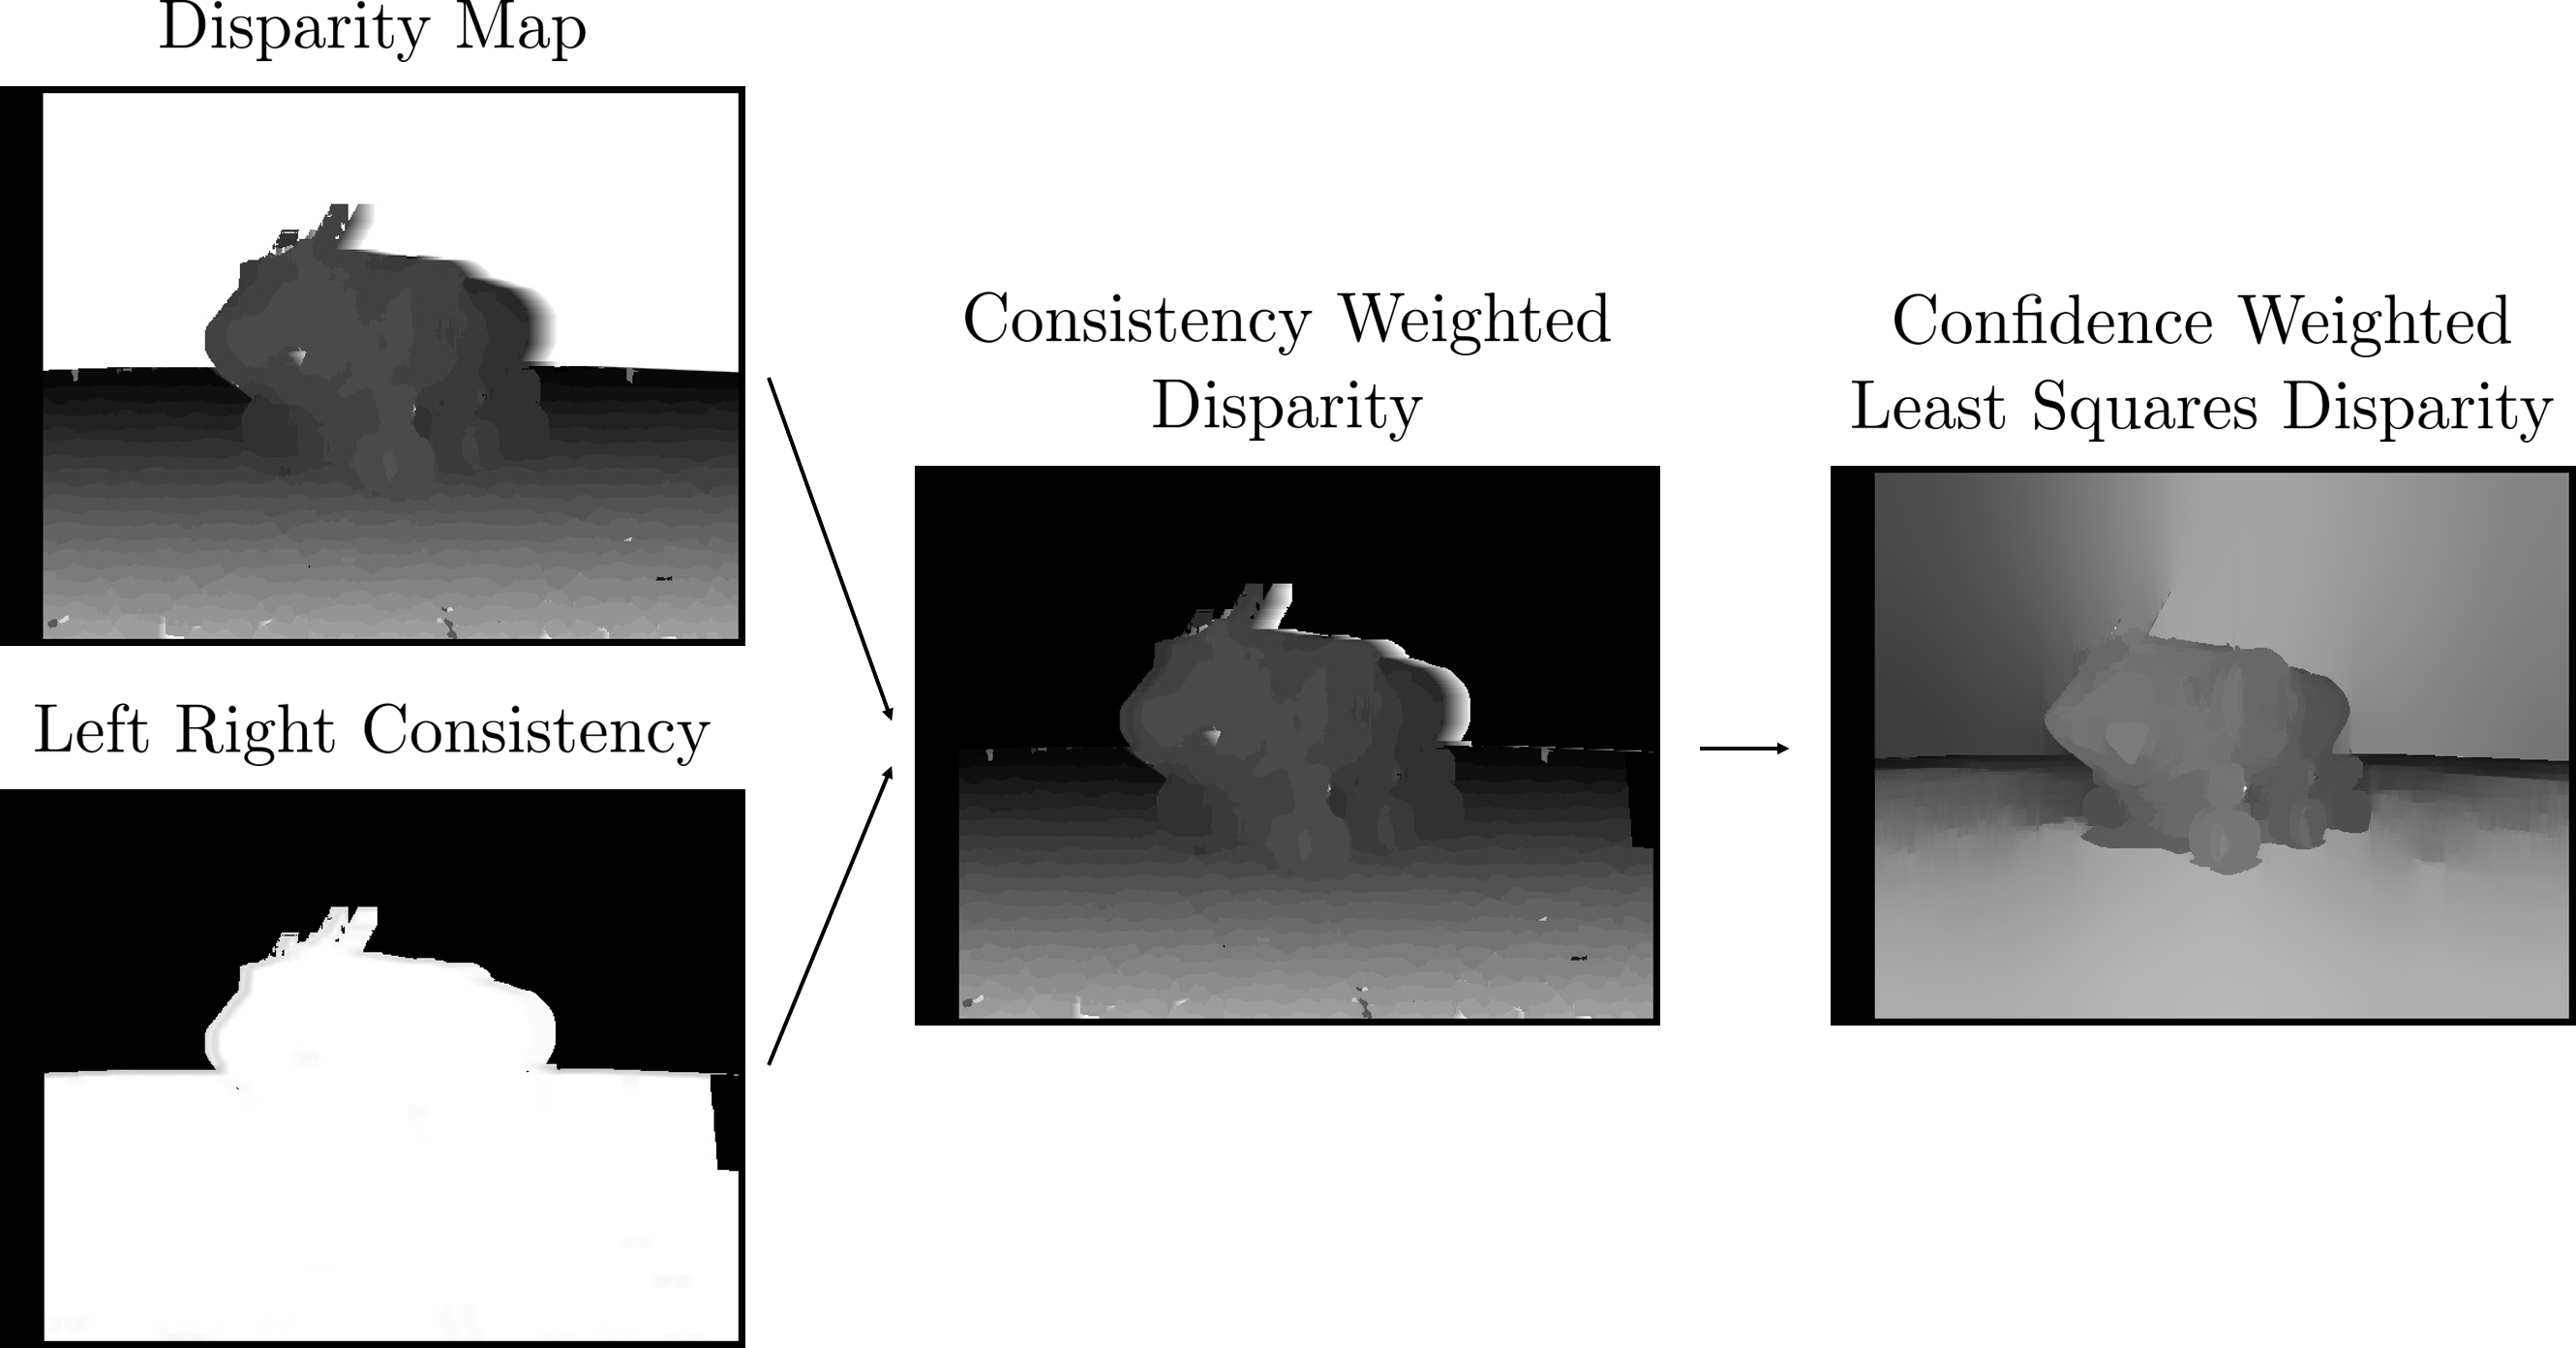
\includegraphics[scale=.28]{chapters/03_background/img/weighted_least_squares_disparity.png}
	\caption{Generation of the confidence weighted least squares disparity from the disparity map, and the left right consistency.}
	\label{fig::323_weighted_least_squares_disparity}
\end{figure}
\\\\
As already mentioned for figure \ref{fig::323_stereo_camera}, the assumption of a simply translated stereo camera pair is almost never correct. In addition, there exist camera intrinsics that deform the observed image, and so the epipolar lines. Therefore, as a requirement for the algorithm to work properly, it is important to calibrate the robot's cameras. The next chapter - Mono and Stereo Camera Calibration, will explain in detail how this is done.
\subsubsection{Mono and Stereo Camera Calibration}
To correct images, as we observe them with a camera, it is required to have a mathematical description of it. A simple one for a camera is the pinhole model, which is shown in figure \ref{fig::323_point_hole_camera}.  
\cite{duane1971close} lense distortion\\
\cite{zhang2000flexible} extrinsic and intrinsic parameter estimation \\
\cite{loop1999computing} rectification??\\
\begin{figure}[h]
	\centering
	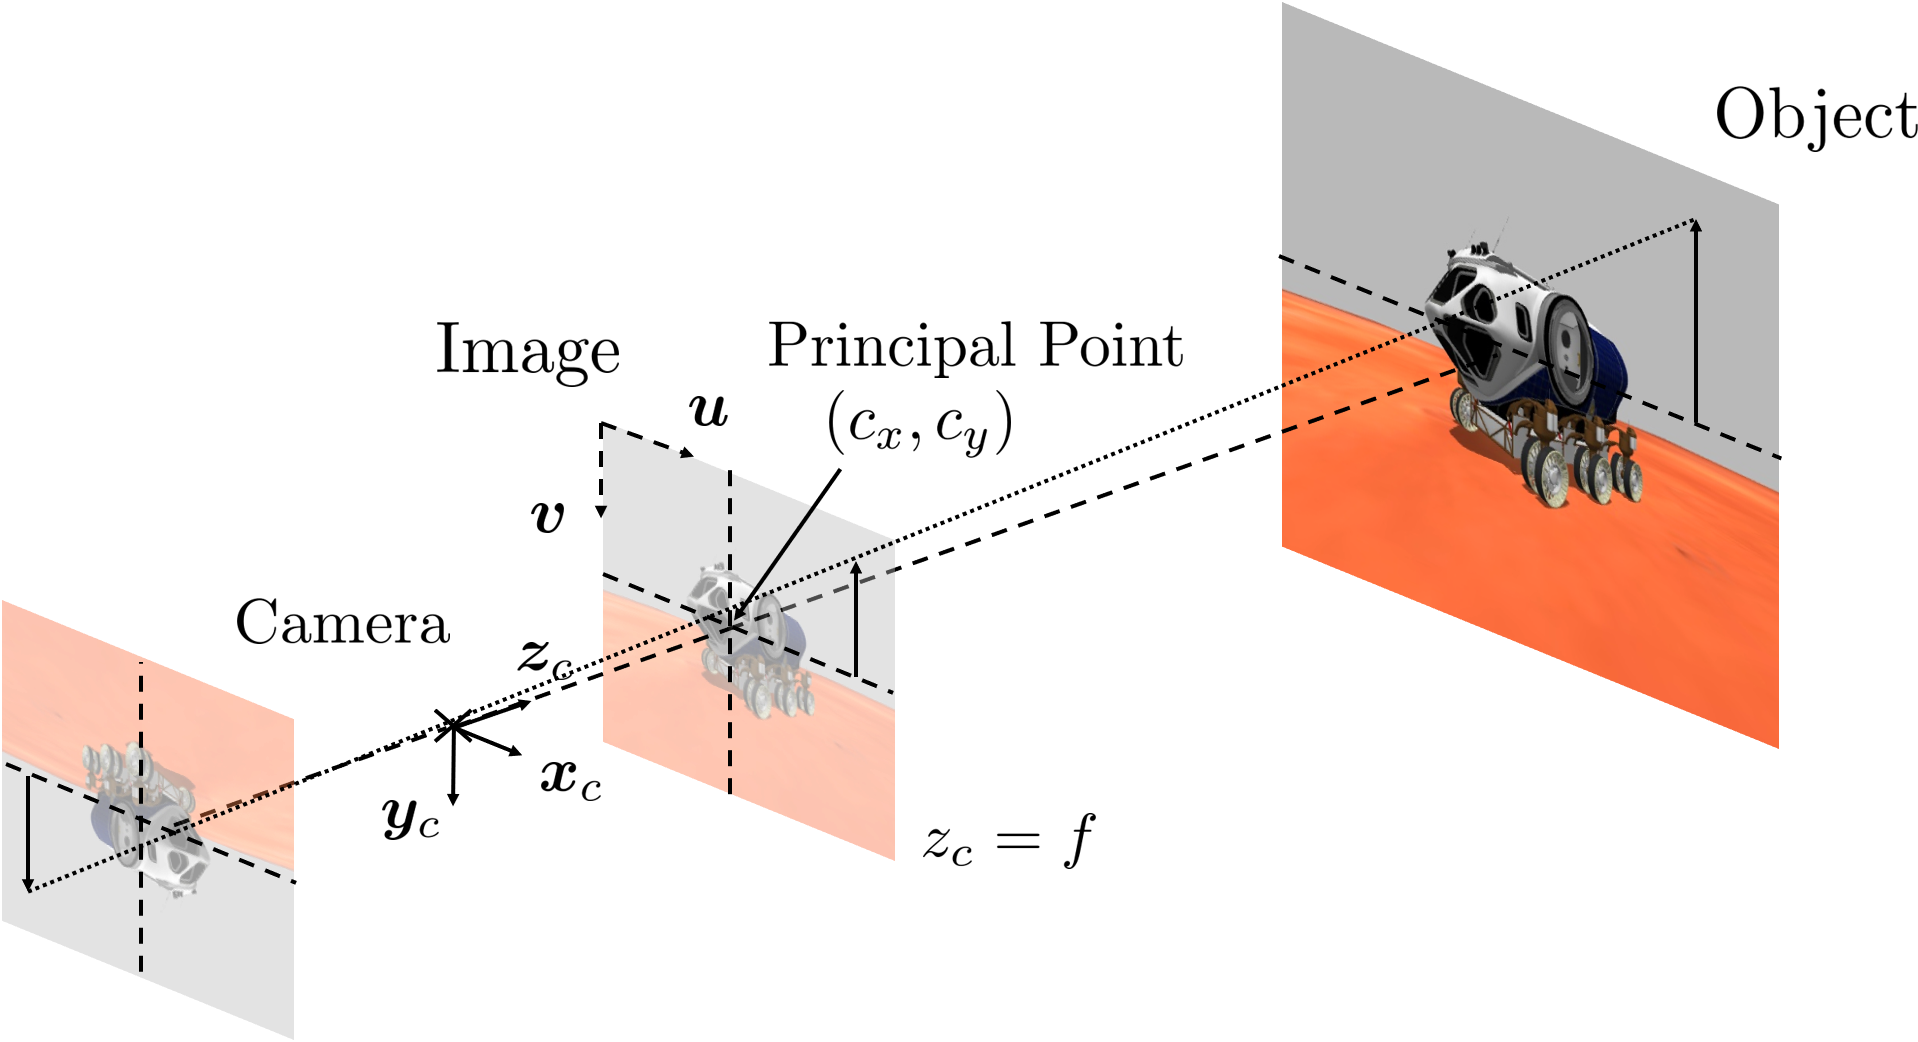
\includegraphics[scale=.28]{chapters/03_background/img/point_hole_camera.png}
	\caption{}
	\label{fig::323_point_hole_camera}
\end{figure}
\begin{figure}[h]
	\centering
	\subcaptionbox{}%
	[.4\linewidth]{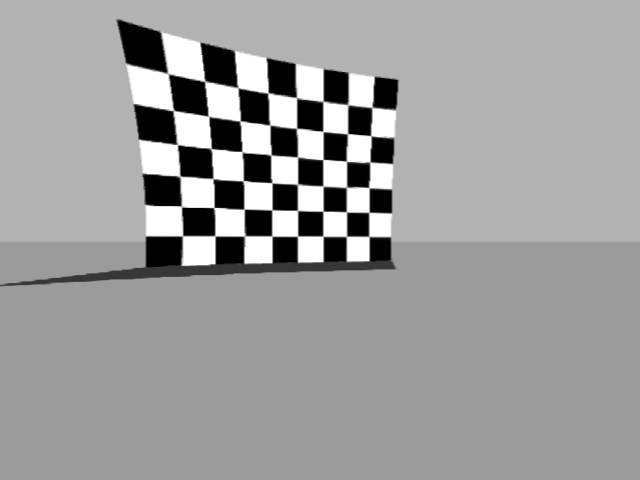
\includegraphics[scale=.2]{chapters/03_background/img/gazebo_calib_left.jpg}}
	\subcaptionbox{}%
	[.4\linewidth]{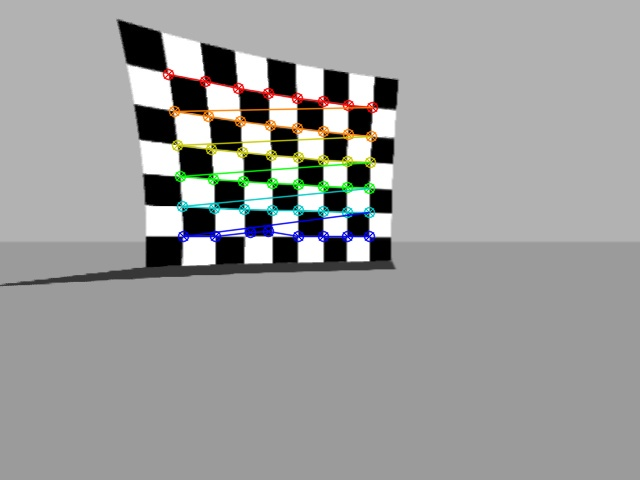
\includegraphics[scale=.2]{chapters/03_background/img/gazebo_corners.jpg}}
	\caption{}
	\label{fig::323_distortion}
\end{figure}
\begin{figure}[h]
	\centering
	\subcaptionbox{}%
	[.4\linewidth]{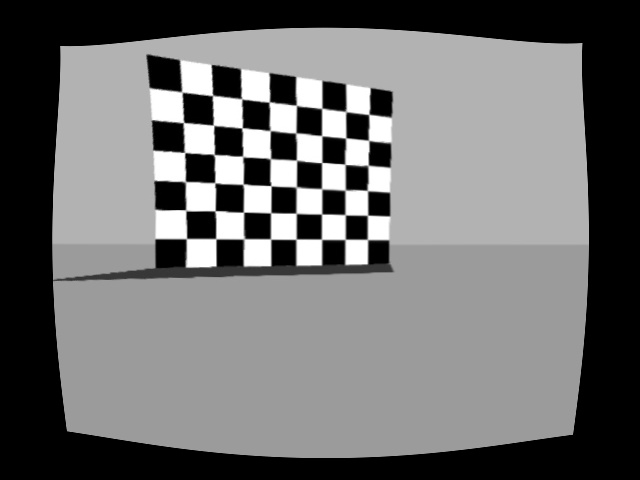
\includegraphics[scale=.2]{chapters/03_background/img/gazebo_rectified_left.jpg}}
	\subcaptionbox{}%
	[.4\linewidth]{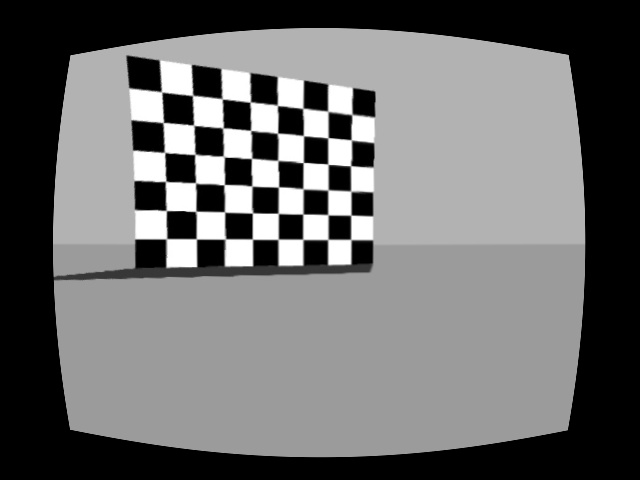
\includegraphics[scale=.2]{chapters/03_background/img/gazebo_rectified_right.jpg}}
	\caption{}
	\label{fig::323_rectified}
\end{figure}
\begin{figure}[h]
	\centering
	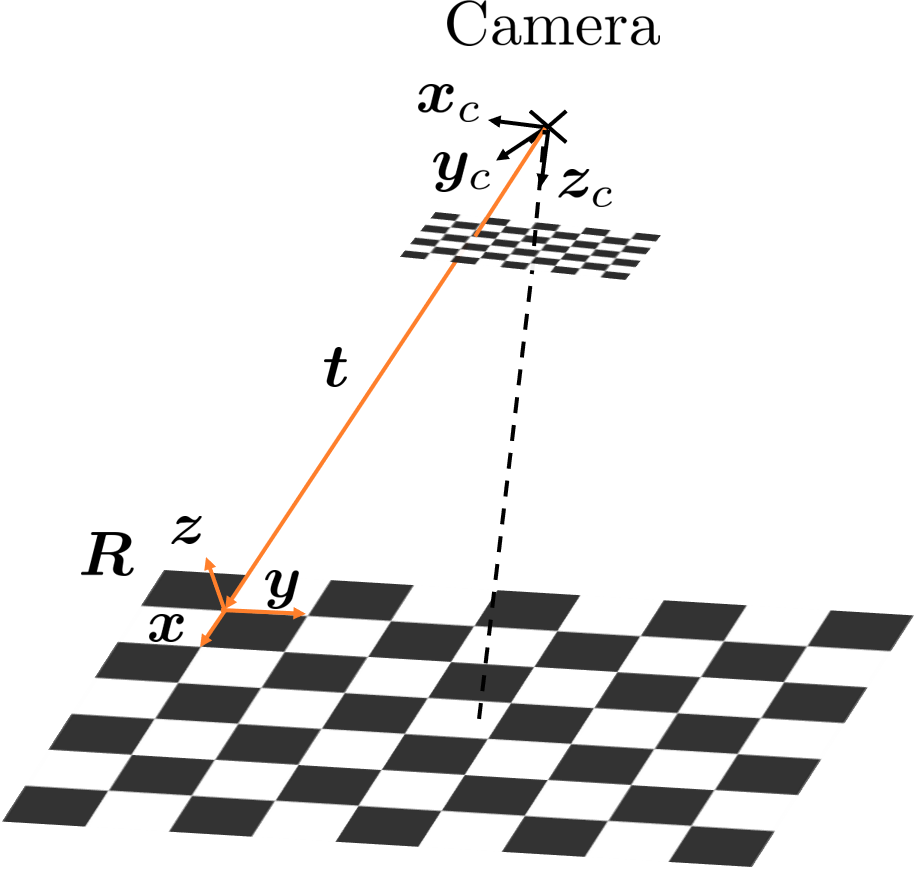
\includegraphics[scale=.28]{chapters/03_background/img/calibration_process.png}
	\caption{}
	\label{fig::323_calibration_process}
\end{figure}